\documentclass{ctexart}

\begin{document}

\title{Test}
\author{wsy}

% 这个是注释
这个是正文

latex命令以反斜杠"\"开始
\usepackage[options]{package}   //相当于#include

行内公式 $x^2+y^2=z^2$    $x^{2+a}_{2n}+y^{2+a}_{2n}=z_{2n}$
整行公式\[
    x^n+y^n=z^n
\]

\begin{equation}
    \[
        D(x)=\dots
    
    \]
\label{eq:equation} 
\end{equation}


LaTex会对插入的公式图表等自动调整编号






插入图片:
\begin{figure}
    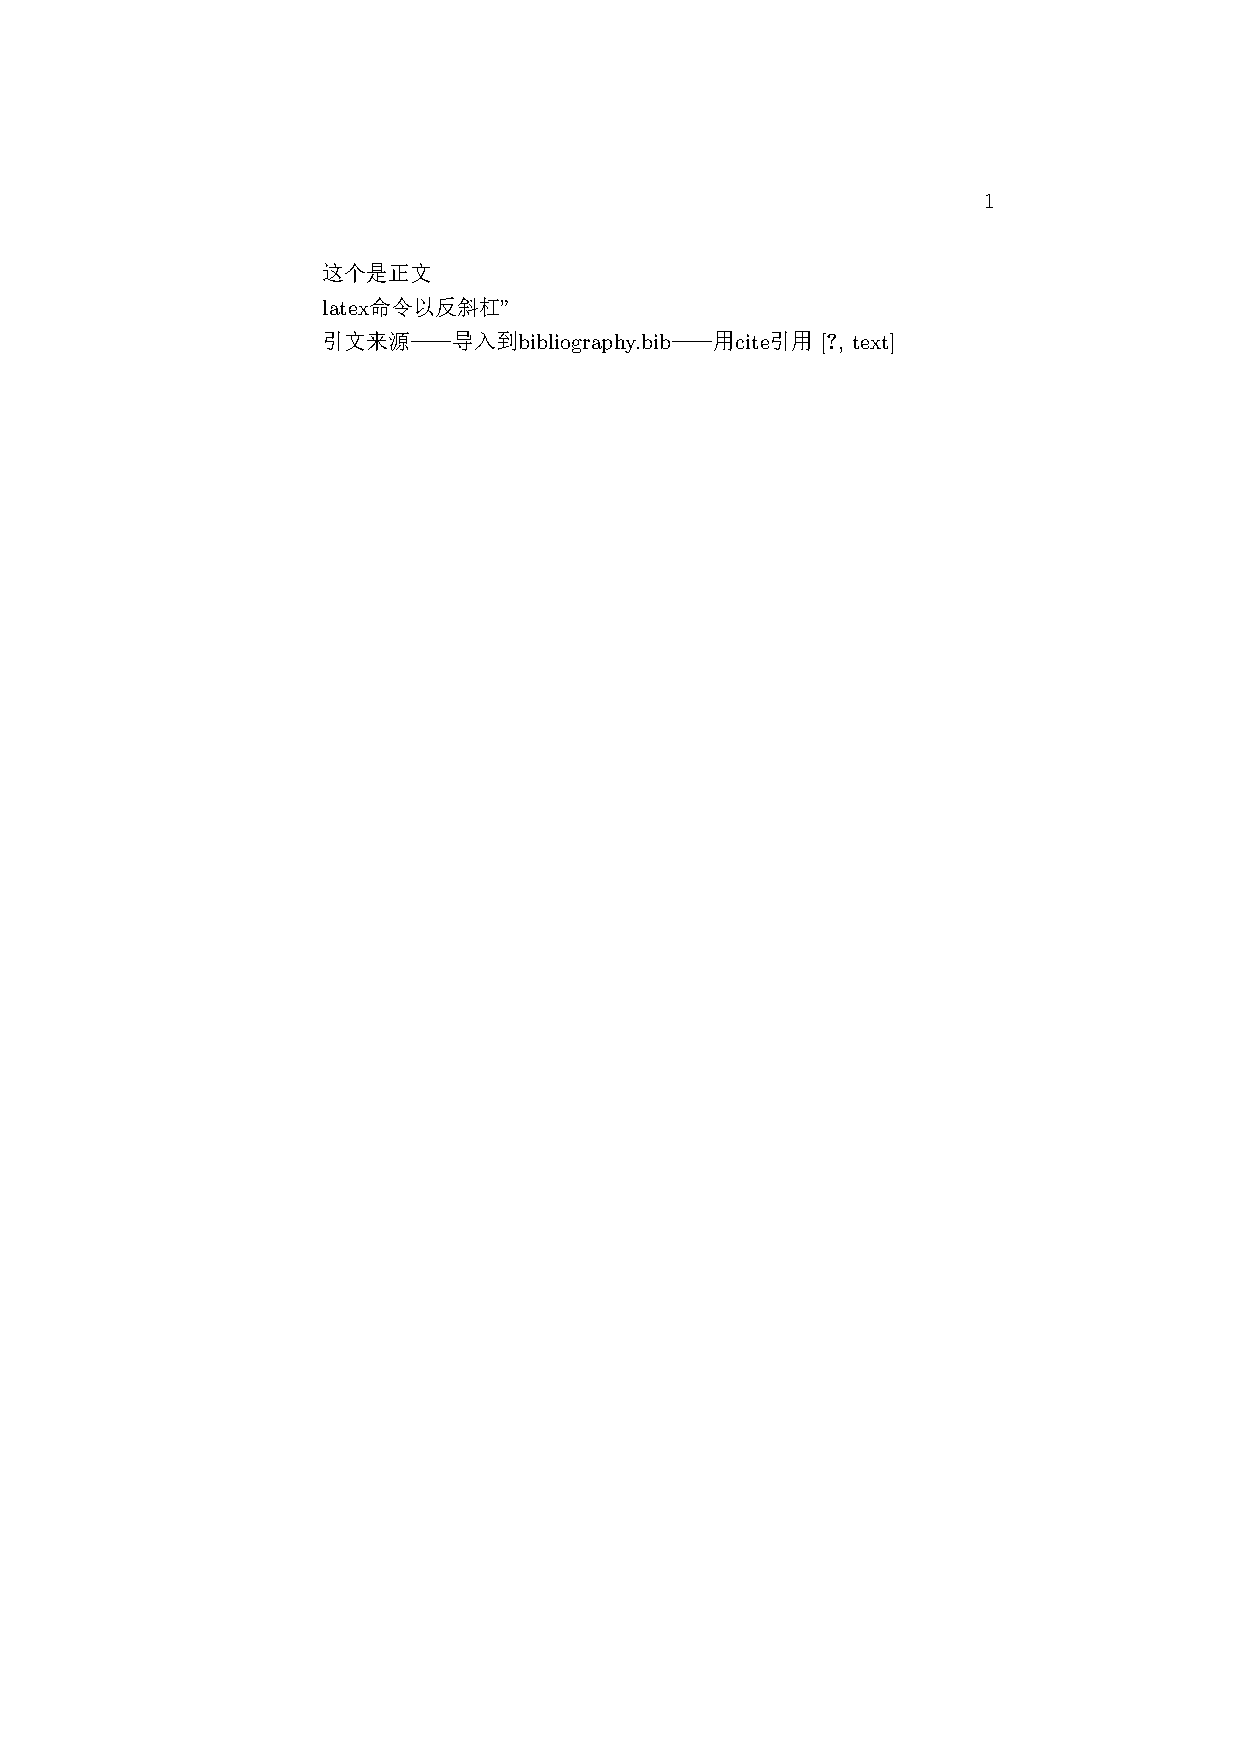
\includegraphics[options(可以不填)]{test.png}
\end{figure}

插入表格:
\begin{tabular*}{width}[pos]{cols}
    \hline
    1 & 2 & 3 \\
    4 & 5 & 6 \\
    7 & 8 & 9 \\
    \hline
\end{tabular*}

引文来源——导入到bibliography.bib——用cite引用
\cite[text]{keylist}





\end{document}